\documentclass[sigconf]{acmart}

\usepackage{booktabs} % For formal tables
\usepackage{gensymb}
\usepackage{graphicx}
\usepackage{enumitem}



% Copyright
%\setcopyright{none}
%\setcopyright{acmcopyright}
%\setcopyright{acmlicensed}
\setcopyright{rightsretained}
%\setcopyright{usgov}
%\setcopyright{usgovmixed}
%\setcopyright{cagov}
%\setcopyright{cagovmixed}


% DOI
\acmDOI{10.475/123_4}

% ISBN
\acmISBN{123-4567-24-567/08/06}

%Conference
%\acmConference[SACMAT'17]{ACM SACMAT conference}{July 2017}{Indianapolis, Indiana USA} 
%\acmYear{2017}
%\copyrightyear{2017}
%
%\acmPrice{15.00}


\begin{document}
%\title{Device Anomaly detection using Provenance Graphs}
\title{  Anomaly Detection in IoT Devices using Provenance Graphs}
%\titlenote{Produces the permission block, and
%  copyright information}
%\subtitle{Extended Abstract}
%\subtitlenote{The full version of the author's guide is available as
%  \texttt{acmart.pdf} document}


\author{Ebelechukwu Nwafor}
%\authornote{Dr.~Trovato insisted his name be first.}
\orcid{1234-5678-9012}
\affiliation{%
  \institution{Howard University}
% \streetaddress{P.O. Box 1212}
  \city{Washington} 
  \state{DC} 
  \postcode{20059}
}
\email{ebelechukwu.nwafor@bison.howard.edu}

\author{Gedare Bloom}
%\authornote{The secretary disavows any knowledge of this author's actions.}
\affiliation{%
  \institution{Howard University}
%  \streetaddress{P.O. Box 1212}
  \city{Washington} 
  \state{DC} 
  \postcode{20059}
}
\email{gbloom@howard.edu}

%\author{Lars Th{\o}rv{\"a}ld}
%\authornote{This author is the
%  one who did all the really hard work.}
%\affiliation{%
%  \institution{The Th{\o}rv{\"a}ld Group}
%  \streetaddress{1 Th{\o}rv{\"a}ld Circle}
%  \city{Hekla} 
%  \country{Iceland}}
%\email{larst@affiliation.org}
%
%\author{Lawrence P. Leipuner}
%\affiliation{
%  \institution{Brookhaven Laboratories}
%  \streetaddress{P.O. Box 5000}}
%\email{lleipuner@researchlabs.org}
%
%\author{Sean Fogarty}
%\affiliation{%
%  \institution{NASA Ames Research Center}
%  \city{Moffett Field}
%  \state{California} 
%  \postcode{94035}}
%\email{fogartys@amesres.org}
%
%\author{Charles Palmer}
%\affiliation{%
%  \institution{Palmer Research Laboratories}
%  \streetaddress{8600 Datapoint Drive}
%  \city{San Antonio}
%  \state{Texas} 
%  \postcode{78229}}
%\email{cpalmer@prl.com}
%
%\author{John Smith}
%\affiliation{\institution{The Th{\o}rv{\"a}ld Group}}
%\email{jsmith@affiliation.org}
%
%\author{Julius P.~Kumquat}
%\affiliation{\institution{The Kumquat Consortium}}
%\email{jpkumquat@consortium.net}

% The default list of authors is too long for headers}
%\renewcommand{\shortauthors}{B. Trovato et al.}


\begin{abstract}

The Internet of Things (IoT) has revolutionized the way we interact with devices. From smart grids, to healthcare and home automation systems. This paradigm shift inadvertently allows for ease of device access. Unfortunately, this technological advancement has been met with unforeseen security challenges. One major challenge is malicious intrusions --A common way of detecting a malicious attack is by treating an attack as an  anomaly and using anomaly detection techniques to pinpoint the source of an intrusion. In a given IoT device, provenance graphs which denotes causality  between system events offers immense benefit for anomaly detection. Provenance provides a comprehensive history of activities performed on a system which indirectly ensures trust. Given a provenance graph, how do we determine if anomalous activities exists? This paper seeks to address this issue. In this paper, We introduce an error tolerant graph embedding technique using frequencies of nodes and edges in which provenance graphs are converted into a vector space representation. This vector space representation of the graphs from learning and detection phase is used as an input  parameter to our anomaly detection algorithm. we propose two anomaly detection algorithms using provenance graphs. The first approach involves the use of a similarity metric to compare provenance graphs while the later involves the use of a hybrid anomaly detection algorithm. We evaluate the effectiveness of our approach with IoT applications which generates provenance graphs.

%We compare our method to two known anomaly detection algorithms. 
\end{abstract}

%
% The code below should be generated by the tool at
% http://dl.acm.org/ccs.cfm
% Please copy and paste the code instead of the example below. 




\begin{CCSXML}
<ccs2012>
 <concept>
  <concept_id>10010520.10010553.10010562</concept_id>
  <concept_desc>Computer systems organization~Embedded systems</concept_desc>
  <concept_significance>500</concept_significance>
 </concept>
 <concept>
  <concept_id>10010520.10010553.10010554</concept_id>
  <concept_desc>Information Science ~Data Provenance</concept_desc>
  <concept_significance>100</concept_significance>
 </concept>
 <concept>
  <concept_id>10003033.10003083.10003095</concept_id>
  <concept_desc>Computer Applications ~Access Control</concept_desc>
  <concept_significance>100</concept_significance>
 </concept>
</ccs2012>  
\end{CCSXML}

\ccsdesc[500]{Computer systems organization~Embedded systems}
\ccsdesc[300]{Computer systems organization~Internet of Things}
\ccsdesc{Computer systems organization~Data Provenance}
 

% We no longer use \terms command
%\terms{Theory}

\keywords{IoT, Data Provenance, Anomaly Detection}


\maketitle

\section{Introduction}
 

Over the years, there has been an increase in the number of intrusions reported on IoT devices. With the pervasive nature of these smart devices, the complexity of intrusions are further exacerbated. Malicious intrusions on IoT devices could have disastrous financial consequences. For example, a vulnerability on a consumer device such as a smart watch or mobile card reader could lead to the theft of sensitive financial and personal information. One way of detecting intrusions is by the use of anomaly detection techniques. An anomaly, also referred to as an outlier, is defined as data that deviates from the normal system behavior. This enables the detection of known and unknown malicious attacks.  Anomaly detection has applications in domains such as intrusion detection, fraud detection, medical health devices, sensor fault detection, web spam. An anomalous event could indicate that a system fault exists. It could also indicate that a system is being used as a botnet in a distributed denial of service attack (DDOS). Due to the sensitive nature of safety critical systems, detecting current and future malicious attacks is of utmost importance to the security of IoT devices. However, ensuring data trust is a challenging task. How do we provide an effective means of detecting anomalous instances in a given system? Provenance can be used to address this issue. Provenance graphs captures a holistic history of system events and also offers an efficient way of representing relationships between multiple data objects which can be used to detect system faults or anomalous system behaviors. For example, sensors deployed in a oil rig, provenance can be used to detect when there is a device leak. Also, in an IoT enabled smart home, provenance can be used to detect a point of intrusion in an event of a system hack. 

In this paper, we motivate the need for device anomaly detection on memory constrained IoT devices. Unlike most anomaly detection system which utilize system call frequencies to detect anomalous system behaviors, We take a different approach to anomaly detection by detecting anomalous system events in IoT devices based on provenance data generated by these devices. We identify how provenance graphs can be used to detect anomalous data instances. We provide an overview of anomaly detection, and provenance graphs. We propose a lightweight graph similarity algorithm for detection of anomalous data instances in IoT devices. This algorithm relies on measuring the similarity of provenance graphs in the learning and detection phase. Our technical contributions in this paper are outlined in detail as follows:



%We also propose a hybrid classification algorithm based on $k$- Nearest Neighbors ($k$-NN), and $k$ means clustering. Anomalous events are detected based on their proximity to known normal provenance graph. Our technical contributions are outlined in detail as follows:

\begin{itemize}[noitemsep,wide=0pt, leftmargin=\dimexpr\labelwidth + 2\labelsep\relax]

\item We introduce a graph-vector space approach to representing provenance graphs in vector space. This allows the comparison of graphs using similarity metrics such as cosine similarity or jaccard distance.



%\item We take a hybrid approach to anomaly detection by combining clustering, classification, and density-based techniques. In the training phase, the unlabeled data set is clustered into two groups (where $k \lesssim 2$). The density of each cluster is observed using the Local Outlier Factor (LOF) to determine which cluster is considered the normal or an anomaly. In the test phase,  $k$ nearest neighbor algorithm is used to classify incoming data instances as normal or anomaly.

\item We propose two anomaly detection techniques for IoT devices using provenance graphs. The first algorithm is based on the similarity between provenance graphs contained in both the learning and detection phase which is achieved by using a similarity metric. A threshold is set which classifies a provenance graph as anomalous once the threshold is exceeded. The second algorithm is a hybrid approach which involves the uses of clustering algorithm, DBSCAN, and $k$-nearest neighbor algorithm, $k$-nearest neighbor.



\item Finally, we evaluate the effectiveness of our approach to graph based anomaly detection with data set from sample IoT application(s). Detailed results are presented in sections IV.

%We calculate the Receiver Operating Characteristic curve. The ROC curve is a measure of the detection rate against the false alarm rate.

\end{itemize}

The remaining portion of this paper is organized as follows. In Section 2, we discuss background information on Anomaly detection, Provenance Graphs, text based query ranking and a review of $k$-NN. In Section 3, we discuss how provenance data is converted in vector space using tf-idf. Section 5 talks about our classification approach using $k$-NN. Section 6 describes our experiment and gives a detailed evaluation. We summarize and conclude in Section 7 and Section 8 contains further discussions.



%Graph based anomaly detection has been explored in various research.Most of the prior work focuses on static graphs using community outliers, and finding similarities from frequent substructures. 

%There are two major approach to intrusion detection. Signature based Intrusion detection and anomaly based detection.

%In recent years,the Internet of Things (IoT) has gathered significant traction which has led
%to the exponential increase in the number of devices connected to the internet. %IoT involves the connection of heterogeneous devices with sensing and actuating capabilities over the internet. 
%It has revolutionized devices to device communication, which in turn optimizes efficiency and improves the standard of living. According to a report released by Cisco, it is estimated that a total of 50 million devices will be connected to the internet by the year 2020.  With the vast amounts of connected heterogeneous devices, security and privacy risks are increased. Data provenance is instrumental to the security IoT data. Provenance describes a holistic history of operations  performed on a data object from its point of creation. Provenance can be used as a measure to ensure trust and also for forensic analysis in an event of malicious attack. Provenance collection system is of immense benefit to IoT devices however provenance incurs additional storage overhead. Continuous provenance collection has the tendency to generate more data than the data it describes. Work done by Brian et al demonstrates that changes to a source file in the Linux kernel results to two kilobytes of additional provenance data when the kernel is recompiled. Additionally, Figure x displays a graph of the growth of provenance data for a raspberry pi collecting temperature and humidity readings. This sensor reading is stored in CTF format. From the diagram we can see that the data grows rapidly with time. This motivates the need for an efficient pruning technique to reduce storage overhead that might be incurred by including provenance in an IoT application. It is of utmost importance to provide a method of pruning provenance data generated thereby reducing the storage overhead. This requirement is further motivated by the constrained memory and computing power of IoT devices. Pruning can be described as removing provenance data in order to conserve storage. 
% \par In this paper, we propose a fine-grained, policy model for provenance pruning. This model provides an expressive policy language which allows device administrators the flexibility of specifying what provenance data to store.  We argue that policy is an effective way of addressing the data pruning problem created by automatic provenance collection. With access control, we allow the flexibility of deciding what provenance data is discarded thereby eliminating unwanted provenance information. Provenance sometimes generates information that might be considered uninteresting. For example, a system collecting the provenance of system events such as device internal system state might be considered uninteresting to a researcher working on collecting temperature and humidity readings or a device administrator interested on. We implement a proof of concept system using XACML, a fine-grained attribute based access control policy language which evaluates request based on a policy specifications. XACML serves as the foundation for our framework.We compared our performance of the proposed framework with state of the art on provenance pruning (e.g web compression + dictionary). 







%IoT trace is derived in the form of CTF output. This output stream is pruned to reduce storage overhead.
%
%CTF is a binary format that allows dynamic instrumentation trace of a applications written in C/C++. The source code for applications  is compiled with the generated c code that barectf creates for the IoT trace event. 
%
%barectf is chosen for tracing IoT device because it generates ANCI C code which is lightweight and can fit into most microcontrollers.

%This mode can also the further applied for access control on resources in an IoT.
%
%Sensor based access control model for authentication and enforcement of provenance data.


%The \textit{proceedings} are the records of a conference\footnote{This
%  is a footnote}.  ACM seeks
%to give these conference by-products a uniform, high-quality
%appearance.  To do this, ACM has some rigid requirements for the
%format of the proceedings documents: there is a specified format
%(balanced double columns), a specified set of fonts (Arial or
%Helvetica and Times Roman) in certain specified sizes, a specified
%live area, centered on the page, specified size of margins, specified
%column width and gutter size.

\section{Problem Statement}

Given a set of provenance graphs, P = $\{p_1, p_2,...p_n\}$ containing provenance data from both the learning and detection phase, we want detect anomalies that might exist in P.  This involves converting elements in $P$ into a feature vector space. Anomalies are detected by comparing the similarity of graphs contained in $P$ using a similarity metric and also by using a hybrid approach as discussed in section IV


% Anomalies are detected using a hybrid approach which is a combination of clustering and classification algorithms discussed in section IV

\section{BACKGROUND}

This section describes key concepts of Anomaly detection techniques, Provenance graphs, text-based query ranking and $k$-NN. 

\subsection{Overview of Anomaly Detection}

The definition of an anomaly is often domain specific. Hawkins, a primer anomaly detection researcher defines an anomaly as an "observation which deviates so much from the other observations as to arouse that it was generated by a different mechanism \cite{hawkins}. An Anomaly is usually considered to be in isolation from similar data points. The notion of a normal behavior is defined by the average behavior that is depicted where most data points are centered in. Anomaly detection has been researched in a wide variety of fields such as statistics, machine learning, information theory. It has applications in finance for fraud detection, in health care for the monitoring of patient care, in computer security for intrusion detection. For the purpose of this paper, we focus on anomaly detection on memory constrained IoT devices. An anomaly often indicates the presence of a malicious entity or a system fault. For example, an anomaly could be a sudden increase in web traffic of a web server.This could be indicative of a denial of service attack. Additionally, In a critical care health device such a as a pacemaker, an anomalous event could be detrimental to the health of a patient which could result in the loss of lives. 






Most of the work done on anomaly detection is centered on the detection of anomalous behavior in point based datasets. This might ignore the dependent relationship that might exist between data points. Graphs provides a means of modeling complex structures such as social networks, computer networks, DNA sequences. 

The process of determining all anomalous instances in a given dataset or system is a complex task. The challenge in anomaly detection is providing the right feature from a dataset to use for detection. Another challenge exists in defining what constitutes as normal system behavior. There often exist a thin line between what is considered normal system behavior and what is considered an anomaly. In addition, what is considered normal system behavior is constantly evolving. The issue of generating training or test dataset which classifies anomalous  and normal system behavior is a major challenge since not all known anomalous system behavior can be recreated.

Anomaly detection consists of two phase: Learning or training phase and the test or detection phase. In the training phase, the system collects training dataset. This data is considered to be a representation of the system's normal daily activity and free from malicious events. Once training dataset has been collected, the system's activities are further observed. This part is known as the testing phase. In the testing phase,  observed system behavior is compared to the Learning phase to determine is an anomaly exists between the two. A threshold as defined by domain experts is used to determine if the observed data is considered an anomaly.


Anomaly detection involves the use of statistical or machine learning techniques  such as clustering and classification to determine normal or anomalous data instances. Some methods deal with assigning a score to determine the anomaly. Details on anomaly detection techniques are outlined below


\begin{itemize}[noitemsep,wide=0pt, leftmargin=\dimexpr\labelwidth + 2\labelsep\relax]


\item Statistical-based approach: This approach involves the use of parametric and non parametric statistical inference to develop models which are used to determine if a dataset fits a statistical model. Instances that do not fit the defined statistical model are classified as an anomaly. Parametric method assumes the knowledge of a distribution. On the other hand, non parametric distribution does not assume prior distribution knowledge. 

\item Classification-based approach: The main idea in this approach involves building models which use training data set with predefined labels (i.e normal, anomalous) to classify incoming data. Classification works in two phase: training phase and observation phase. In the training phase, data is collected which contains labels of normal and anomalous system behavior. If the dataset only contains a label of either anomalous or normal behavior, this is considered as a one class classifier. In the observation phase, incoming data is classified by defined data labels.

\item Clustering-based approach: The main idea is to group similar data instances into clusters. There are various approach to clustering. One approach looks at the density of the clusters, normal data belongs to large dense clusters while abnormal data belongs to small clusters. Another approach as treats clustering as one class which assumes that normal belongs to a cluster and abnormal data does not. Another approach looks at the distance of the data to the centroid. Centroids are seen as the center of the cluster. Normal data are  considered to be closer to the centroid than anomalies lie


\item Nearest-Neighbor based approach: It is based on the assumption that normal data occurs in dense neighborhoods and abnormal data in sparse neighborhoods. The main idea is to assign an incoming observation data to a class based on its proximity to the closest data point in the training data set. A distance or similarity measure is used to quantify the distance between points in a dataset.  A popular form of nearest neighbor technique is the $k$-nearest neighbor which groups incoming data based on proximity to $k$ closest data point. Details on $k$- nearest neighbors is discussed in section 3.5. 

\item Density-based approach: This approach is used to estimate the density of  $k$ nearest neighbors. A data instance in a dense neighborhood is considered normal while data instances in neighborhoods with a sparse density are considered anomalous. The distance from a data instance to a nearest neighbor is seen as the inverse of the density of data instances.  This approach faces an issue in which the density approach performs poorly in regions of varying densities. Local Outlier Factor (LOF) addresses this issue. LOF is a measure of the degree of Outlieriness of each data instance contained in a data set. It is achieved by comparing the ratio of local density of k nearest neighbors to the density of a data instance. Data instances with lower density are considered outliers.

\end{itemize}    


Data labels are grouped into three major categories. Supervised anomaly detection, semi-supervised anomaly detection, and unsupervised anomaly detection. In supervised anomaly detection approach, training data contains instances of normal and anomalous data. Incoming data is classified based on the training data category. In semi-supervised approach, only one class of training data is collected, normal data. Incoming data that does not fit the normal class as specified by a threshold is regarded as an anomalous. In the training phase, most anomaly detection techniques use data derived from the normal system behavior.  This is referred to as one class classification. In unsupervised approach, there are no training dataset. it is believed that normal data is clustered around each and occurs more frequently than an anomaly. This is a widey used form of anomaly detection since training data which is hard to get is not requited. Detailed information on anomaly detection techniques can be seen in \cite{chandola_anomaly_2009, Akoglu2015, hodge_survey_2004, zhang_outlier_2010}

 





\subsection{Provenance Graphs}

Provenance denotes the origin of an object and all other activities that occurred. An example of provenance can be seen with a college transcript. A transcript is the provenance of a college degree because it outlines all of the courses satisfied in order to attain the degree. In the field of computing, data provenance, also known as data lineage, can be defined
as the history of all activities performed on a data object from its creation to its current state. Provenance ensures trust of data \cite{Bertino2015}. It outlines causality and dependency between all objects involved in the system and allows for the verification of a data source. In and IoT device, a provenance graph $G= (V, E)$ is a directed acyclic graph (DAG) in  which vertices represents device or sensor events data and the edges corresponds to the interaction between them 

Graphs provide a means of modeling complex relationships that exits between data objects and is a good choice for modeling provenance because provenance data contains information with dependency relationships which denotes causality between multiple data objects. Provenance data is represented by directed acyclic graphs where nodes denote data objects and the edges represent relationships between data objects. For example, provenance graph from a device can be generated  by evaluating the log of system calls. This log information might contained noisy data and is further streamed by mapping it to a provenance model. With this information, we are able to build a workflow of device data execution. There has been numerous provenance collection systems developed to track provenance in a computing device most of which deals with tracking system calls \cite{pasquier-socc2017,acsac,Muniswamy-Reddy}. Provenance graph used for experimentation is generated from PAIoT, a provenance-aware framework  \cite{} . We chose PAIoT because it captures dependencies between device and sensor events. 

\begin{figure}[h!]
\begin{center}
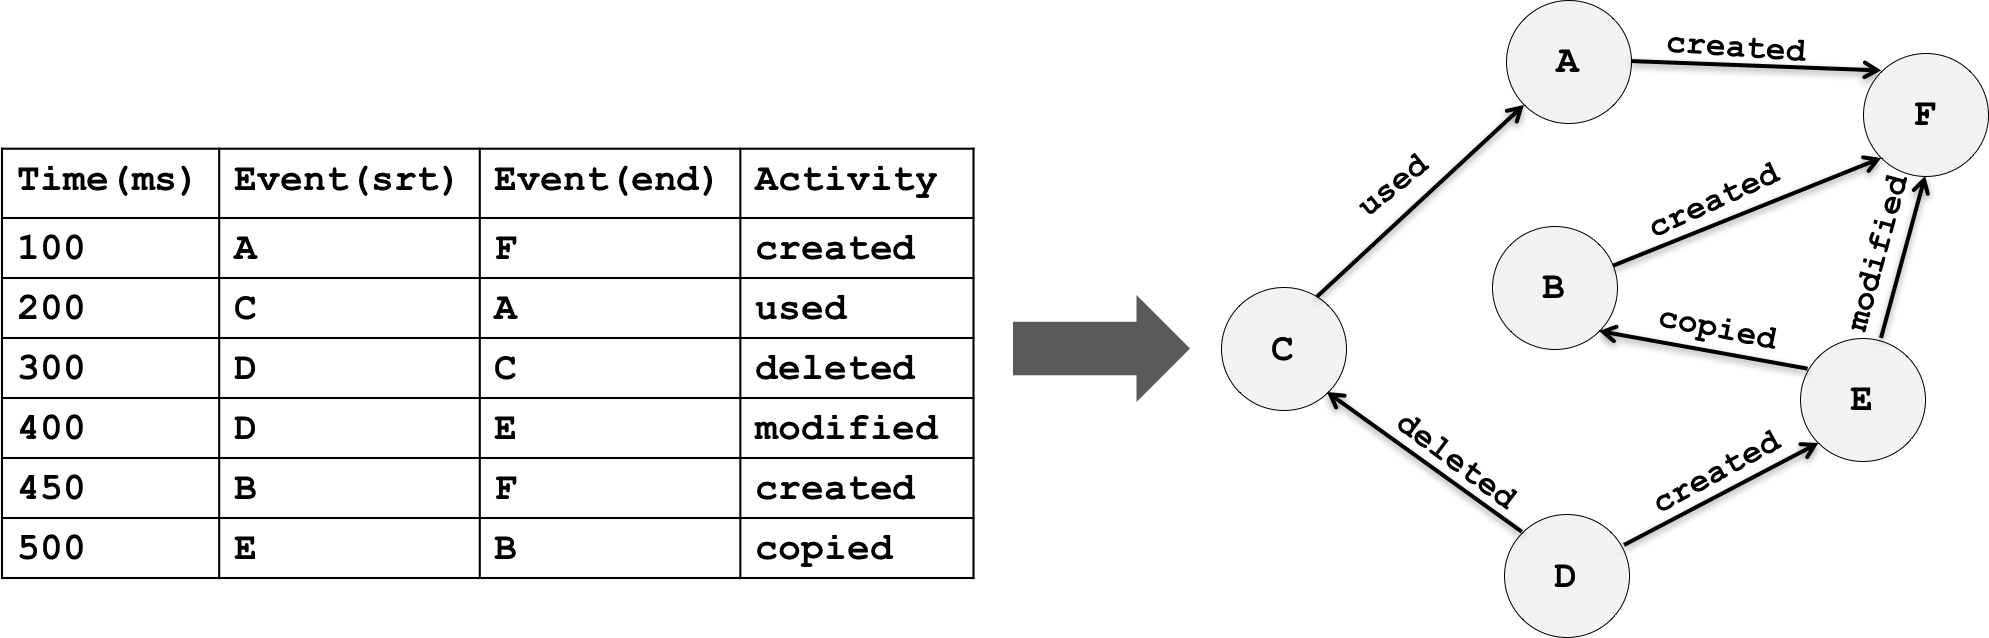
\includegraphics[height=1.4in, width=3.5in]{provenance_graph_2.png}
\end{center}
\caption{Provenace data transcribed to Provenance graph which depicts causal dependency between system events. The nodes represents events while the edges represents activities}
\label{Provenance_graph}
\end{figure}

 


Causality and dependency are concepts used to denote relationship between system events. Provenance graphs in turn be used in digital forensics \cite{zhang_outlier_2010} to investigate the cause of a malicious attack and also in intrusion detection systems to further enhance the security of computing devices. For further reading on provenance models and provenance graphs, we refer the reader to \cite{}  


 





%\subsection{Provenance-system collection}
%
%\subsubsection{Observed Provenance}
%
%\subsubsection{Disclosed Provenance}



%\subsection{Provenance Characteristics}
%
%Since provenance denotes the who, where and why of data transformation, it is imperative that data disseminated in an IoT architecture satisfies the required conditions. The characteristics of data provenance are outlined in detail below.
%
%
%\begin{itemize}
%
%\item Who: This characteristic provides information on activities made to an entity. Knowing the ``who" characteristic is essential because it maps the identity of modification to a particular data object. An example of ``who" in an IoT use case is a sensor device identifier.
%
%\item Where: This characteristic denotes location information in which data transformation was made. This provenance characteristic could be optional since not every data modification contains location details.
%
%\item When: This characteristic denotes the time information at which data transformation occurred. This is an essential provenance characteristic. Being able to tell the time of a data transformation allows for tracing data irregularities.
%
%\item What: This characteristic denotes the transformation is applied on a data object. A use case for IoT can be seen in the various operations (create, read, update, and delete) that could be performed on a file object.
%
%\end{itemize}
%
%
%There are two ways of pruning Provenance data: Provenance can be pruned at collection before it is been committed to the disk  or after being recorded to disk. Policy defines rules and actions that should be taken if any of the rules applies.  Access control in this case is used as a tool for pruning provenance data stored on an IoT device. It can also be extended for traditional access control measures. Data pruning is an essential problem for automatic provenance collection. Observed provenance and disclosed provenance. Observed provenance involves automatic collection of system states and changes. One major drawback of this method is that all system events are provenanced including irrelevant system provenance which incurs more storage overhead. Described provenance on the other hand, allows a user to provide a workflow of how what provenance the system is intended to generate and an engine to execute the workflow described.

%\subsection{ Document retrieval using vector space model} 
%Vector space conversion is used in information retrieval technique for determining document similarity to a query. Given a corpus $D = \{ d_1,..., d_n\}$, a query, $q$,  find document(s) ${d_x,....d_y}$ which are similar to $q$ and rank them by order of importance. To achieve this, documents are converted into a vector space representation which allows document to be ranked based on some similarity metric.
%
%
%\subsubsection{term frequency-inverse document frequency:}
%
%term frequency - inverse document frequency (tf-idf) is a widely used weighting scheme for ranking documents in a corpus given a query. The algorithm reflects how important a word is to a document. The more common a word is in a document, the higher the weighting factor. Given a term $t$ in document $d$ the term frequency $tf(t,d)$ is the number of times $t$ occurs in $d$.  tf-idf is composed of two algorithms: term frequency $tf$ and inverse document frequency, $idf$ .  tf-idf is derived from the product of tf and idf.
%
%  \[ tf-idf(t,d, D) = tf(t,d) \times idf(t,D) \]
%
%\par There are a number of ways to calculating the term frequency of a document. The first approach counts the raw frequency of each word contained in the document. 
% 
%
%\[ tf(t,d) = freq(t,d) \]
%
% 
% Another approach is to use boolean weighting. If a word is contained in a document, a weight of 1 is assigned as the term frequency, otherwise, a weight of 0 is assigned.
% 
% Other ways of computing the term frequency involves the use of the normalized instances of the term frequency. (i.e by dividing the frequency of each words by the total number of words contained in the document or by using the log of the raw frequency)
%
%  \[ tf(t,d) = \dfrac{freq(t,d)}{N} \]
%  
%   
% \[ tf(t,d) =  \log{(freq(t,d))} \]
% 
% 
%One major drawback of using the term frequency is that all terms in a document are considered equal while retrieving a query.In a corpus, some documents might contain words that are commonly repeated in every other documents. This adversely influences the weighting factor of a term in a corpus. For instance, in a collection of documents, words like  "the" are widely used and might occur more frequently.  Inverse document frequency (idf) ensures that frequently occurring words in a list of documents are given a lower weight than less occurring words. The more frequent a term occurs in a corpus, the less the idf weight.
%
% idf is computed by taking the log of the total number of documents in a corpus , $N$ divided by the number of documents which contains the term $df_t$.
% 
% \[idf(t, D) =\log \dfrac{N}{df_t} \]
% 
%tf-idf weighting scheme provides a vector space representation of documents. To compare the similarity between two documents, we employ the use of  a similarity measure such as cosine similarity, Jaccard similarity or euclidean distance. This similarity measures calculates some form of distance between the two vectors. Cosine similarity has been shown to outperform the rest of the similarity measures in comparing documents.

\subsection{Similarity Measures}
Similarity defines how identical two objects are. It measures some form of distance between data objects by either measuring the angle between the objects (Cosine similarity) or a linear distance between the objects (Euclidean distance). Similarity measures are widely used in document retrieval for selecting a query given a list of documents. The similarity measure used is application dependent on the data set and the sparsity of data. Based on literature, there are three well known similarity measure for evaluating vectors. These measures are outlined below:

\subsubsection{Cosine similarity:}

This is a measure of orientation between the two non-zero vectors. It measures the cosine of the angle between the vectors. Two vectors which are at an angle of 90\degree  have a similarity of 0 while two vectors which are similar (with an angle of 0\degree) have a cosine of 1 and two vectors which are completely opposite (with an angle of 180\degree) have a similarity of -1. Since we are concerned with the similarity of the vectors, we are only concerned with the positive vales of bounded in [0,1]. To compute the cosine similarity between two vectors, $X$ and $Y$, cosine similarity is represented by using the dot product and magnitude of the two vectors.

\[\mathbf{\cos{(\theta)}} = \dfrac{X \cdot  Y}{ \lVert \mathbf{X} \rVert \cdot \lVert \mathbf{Y} \rVert} =\dfrac{\sum_{i=1}^n X_i Y_i }{\sqrt[]{\sum_{i=1}^n X_i^2} \sqrt[]{\sum_{i=1}^n Y_i^2}}  \]

\subsubsection{Jaccard Similarity:}
This similarity measure evaluates the intersection divided by the union of two non zero vectors.


\[ J(A,B) = \dfrac{|A \cap B | }{| A \cup B |} \]

\subsubsection{Euclidean distance:}
This measures calculates the line distance between two data objects in an euclidean space. The euclidean distance between vectors $A$ and $B$ , $d(A, B)$ is defined by: 

\[ d(A, B) =  \sqrt{\sum_{i=1}^n (A_i - B_i)^2} \]




\subsection{A Review of $DBSCAN$ and $k$-nearest neighbors}

\subsubsection{$k$-Nearest Neighbors:} $k$-NN is an instance based supervised learning algorithm for classifying data based on nearest neighbors. Data is grouped on its similarity to nearest neighbors where $k$ denotes the number of neighbors in which the input data is compared to.  A similarity measure such as euclidean distance, jaccard similarity, or cosine similarity is used to measure the distance between vectors. $k$-NN can be applied to classification and regression problems.

Researchers have proposed various modifications to the $k$-NN algorithm. Ramaswamy et al. \cite{Ramaswamy} proposed a $k$-NN modification which calculates the sparseness estimates for vectors in a dataset. The vectors are sorted in increasing order according the distance from its $k^{th}$ neighbor. Bay and Swabacher demonstrates how pruning irrelevant datapoint which are not considered anomalous can result in a linear complexity of nearest neighbor search for a randomized data. A threshold score is assigned which is based on the score of the weakest anomaly found. Pruning can be achieved by using the  relative density of data points, an anomaly is believed to occur in a group of data points with low density.

\subsubsection{Density Based Spatial Clustering of Applications with Noise ($DBSCAN$):}

\textit{DBSCAN} is a density-based clustering algorithm that differentiates regions with high density from regions with low density. It defines two parameters $\boldsymbol{\epsilon}$, and $\boldsymbol{MinPts}$. $\epsilon$ defines the maximum distance between two neighboring points in which they are considered to be in the same cluster. $MinPts$ is the minimum number of points that can be contained in a cluster. 

Let $S = \{s_1, s_2,...s_n \}$ be a set of point to be clustered. $S$ consists of three point categories, a core point, $\boldsymbol{p}$, a border point, $b$ and a noise point, $n$. A core point is a point in which its $minPts$ are within distance $\epsilon$. These are at the interior of the cluster. Border points are points on the edge of the cluster. A noise point (outlier) is any point that is neither a core point or a border point.

A point, $l$ is directly reachable from a core point, $p$ if there exist a path which is within distance of $\epsilon$ from the core another point. (i.e $ \exists \quad  \{p_1, p_2,...p_n \},\quad \textrm{where} \quad |p_{i+1}  - p_i| \leq \epsilon$ ). 



A core point, $\boldsymbol{p}$ that is within distance $\epsilon$ (i.e $p \leq \epsilon$) is considered part of the same cluster. A border point is also considered part of a cluster if it close to a core point. 


%\subsubsection{ $k$ means clustering:}




\section{Graph Based Anomaly Detection }

\subsection{Potential Anomalies}

Due to the ubiquitous nature of IoT devices, there are a wide array of potential vulnerabilities associated with them. We focus on select vulnerabilities of inconsistent sensor output. Inconsistency are analogous to spikes in sensor readings, constant data values, or faulty sensors, inconsistent device attributes.





\subsection{Graph to Vector Space Conversion }

\subsubsection{Feature Extraction}

In order to apply clustering algorithms or similarity measure to provide anomaly detection, we compute a vector space representation of our provenance graphs. This representation is used as input parameters to our hybrid anomaly detection algorithm. Selecting features from graph properties is an important task because we need to select features that preserves the order and details of each node and edges contained in the graph. We focus on the frequency of the nodes and edges contained in both graphs. Selecting the right features is important in ensuring optimal performance of our anomaly detection algorithms. Our approach not only utilizes the frequency of nodes but also consists of a damping factor which regulates the weight of nodes or edges that occur frequently and increases the weight of nodes and edges that occurs less frequently.  
 

\par Given a set of provenance graphs $P = \{p_1,....p_n \} $, where $p_x = (V, E)$. $P$ consists of graphs both in the learning and detection phase. We denote the occurrence of edges and nodes contained in set $P$. Each graph in $P$ represents a vector by using our graph embedding approach which draws emphasis from document query retrieval. This approach preserves the order of edges and allows updates of edges of incoming graphs. We  formally define our approach as follows:


\begin{definition}

Let $P = \{p_1,...,p_n\}$ where $p_i = (V, E)$, the vectorial representation of $p_i, v_{i}$ is the number of times each vertice, $V_i$ and edges, $E_i$ contained in $P$ appears in the graph , $p_i$.

\[ \boldsymbol{v_x} = ( freq(E_i, p_i), freq(V_i, p_i)) \]

where $freq$ denotes the occurrence of $E_i$ in graph $p_i$

\end{definition}

The order of Edges and vertices can be found by taking a breadth first search transversal of the graphs.


\begin{figure}[h!]
\begin{center}
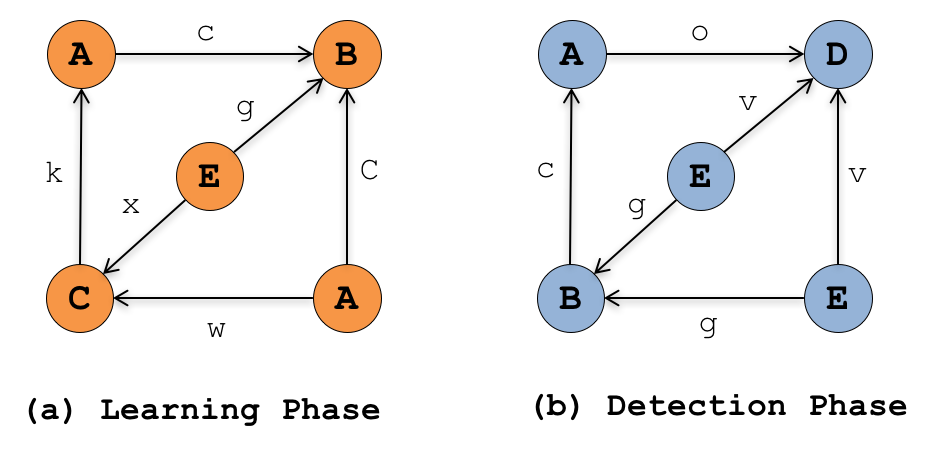
\includegraphics[height=1.7in, width=3.5in]{graph_sim.png}
\end{center}
\caption{Two graphs one generated from the Learning phase and the other from the Detection phase}
\label{example}
\end{figure}


For example, Figure \ref{example} displays provenance graph generated in the Learning and detection phase respectively. Both graphs, $\boldsymbol{p_1}$, and $\boldsymbol{p_2}$ consists of vertices $A,B,C,D, and E$.  The vector representation of the two graphs, $v_1$, and $v_2$ are 

\[ \boldsymbol{v_1} = (1,1,1,1,1,0,0) \] \[\boldsymbol{v_2} = (1,2,0,1,1,1,0) \]









\subsection{Graph Based Similarity Detection Algorithm}

%Talk about how this method preserves the order of edges and also prove that isormophism is preserved. 

The method of comparing the similarity of graphs based on a similarity metric is inspired by a document retrieval technique. Given a corpus $D = \{ d_1,..., d_n\}$, and query, $q$,  How do we find document(s) ${d_x,....d_y}$ which are similar to $q$ and rank them by order of importance. To achieve this, documents are converted into a vector space representation which allows document to be ranked based on some similarity metric. Figure \ref{graph_similarity} depicts the overall goal of the similarity approach in detecting anomalies.


\begin{figure}[h!]
\begin{center}
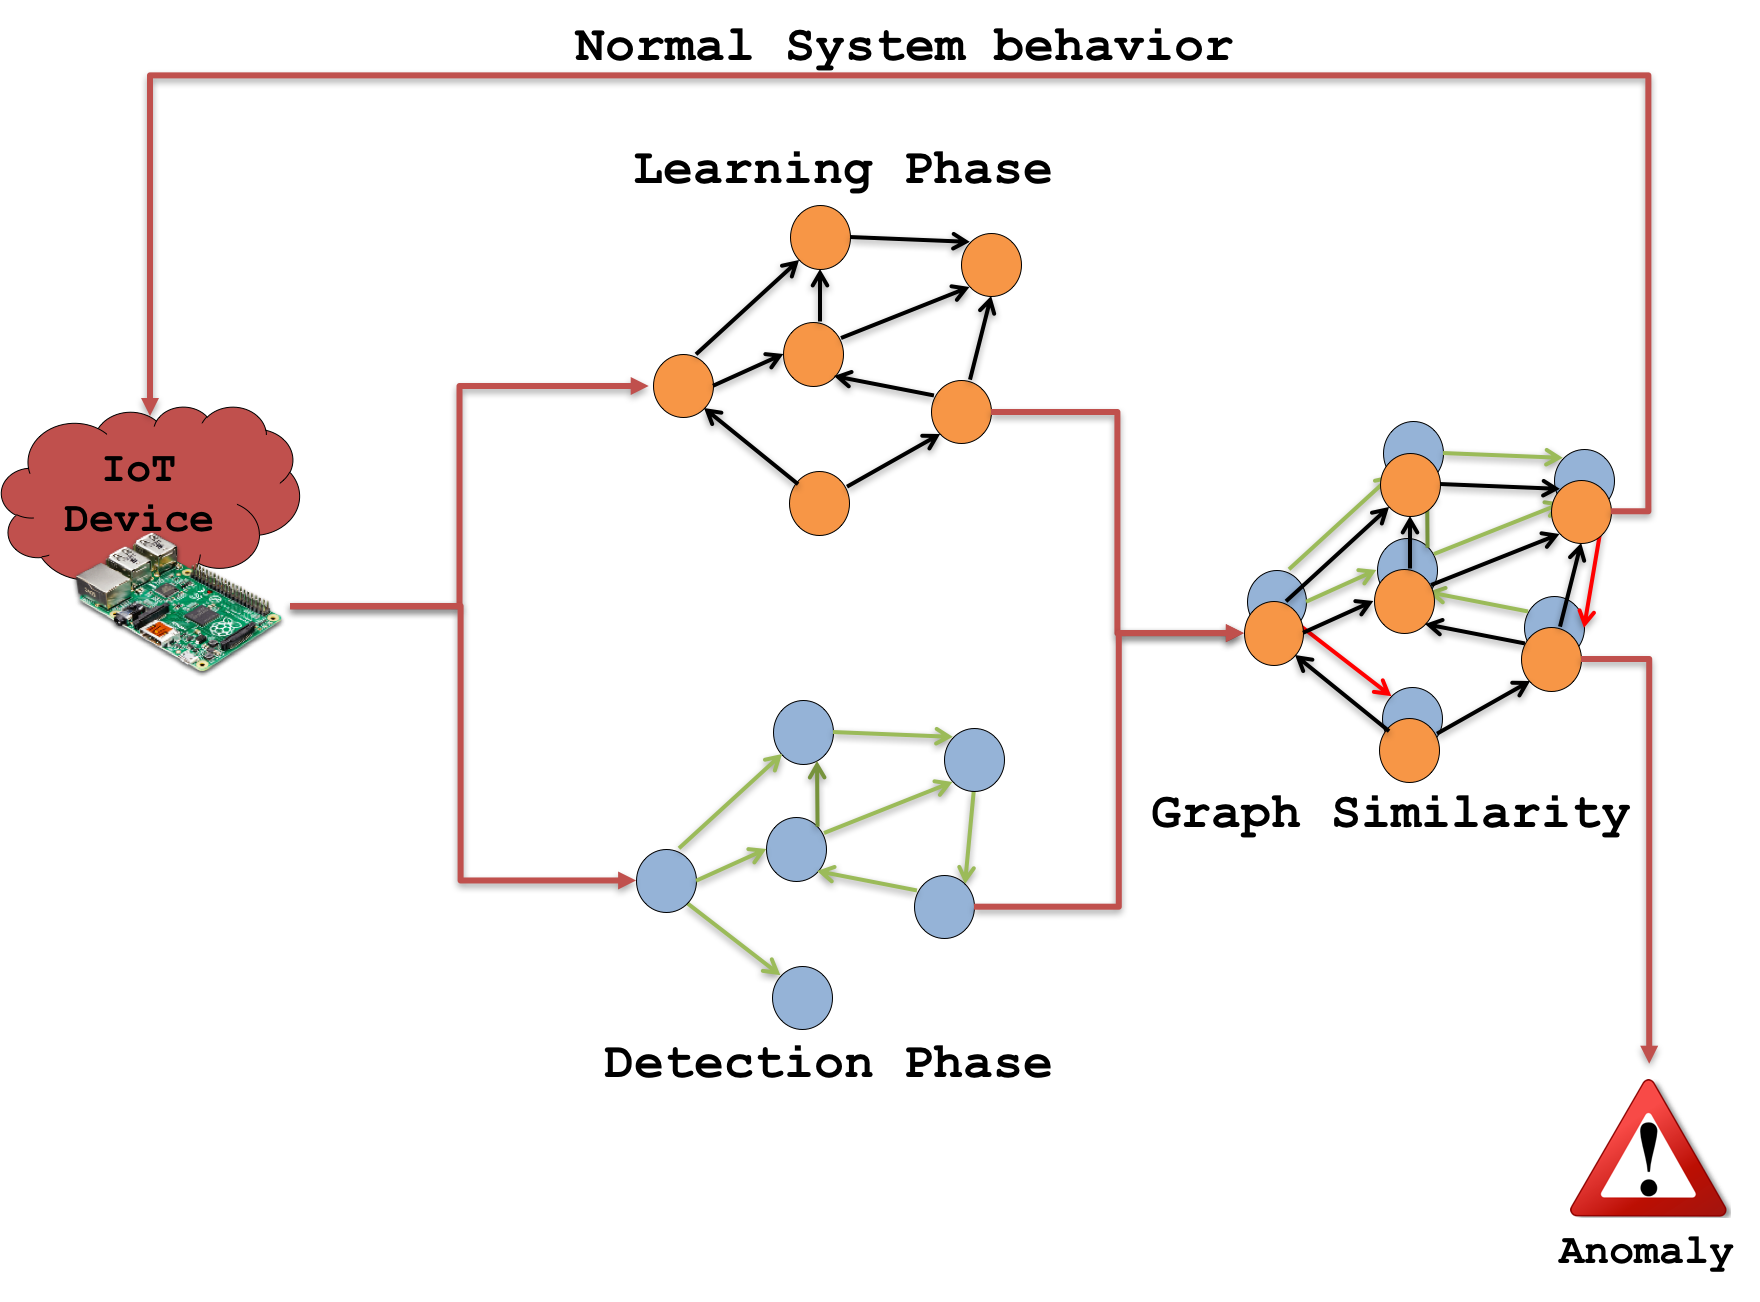
\includegraphics[height=2.5in, width=3.5in]{similarity_5.png}
\end{center}
\caption{Graph Similarity Approach}
\label{graph_similarity}
\end{figure}

Given $v_x, v_y$ which denotes the vector representation of provenance graphs $p_x, p_y$. The similarity of $p_x, p_y$ is found by calculating the cosine similarity between the two vectors where 1 denotes similarity between the two vectors and 0 denotes non-similarity between the two vectors. A threshold value is set which is used to classify the behavior of provenance graphs in the detection phase as normal or an anomaly.

\[sim(v_x,v_y) =  \dfrac{v_x \cdot  v_y}{ \lVert \mathbf{v_x} \rVert \cdot \lVert \mathbf{v_y} \rVert} =\dfrac{\sum_{i=1}^n v_{xi} v_{yi} }{\sqrt[]{\sum_{i=1}^n v_{xi}^2} \sqrt[]{\sum_{i=1}^n v_{yi}^2}}  \in [0,1] \]




\subsubsection{Defining Anomaly Threshold:}

An anomaly threshold $t$ is a score that defines at what point a provenance graph contained in the test data is considered anomalous. Ensuring a proper threshold score is used for detection is an important task that requires extensive knowledge of the attack domain. The threshold is manually set to a value t, which is defined by domain experts. For automatic anomaly threshold detection, one can use forecasting methods to define the anomaly score. Forcasting techniques are beyond the scope of this research. 

\subsubsection{Computational Complexity:}

\textcolor{red}{  TODO}

\subsection{Hybrid Detection Algorithm}

\textcolor{red}{TODO...}



\section{Experimental Evaluation}

\textcolor{red}{TODO...}


\section{Related Work}

There has been a considerable amount of research done on anomaly detection. Most of the work which involves the analysis of system call events. Liao et al \cite{liao_using_2002} characterizes a system's normal behavior by denoting the frequency of unique system calls which are converted to a vector space using the text classification approach. A classification algorithm $k$-NN is used to classify test data set. Our approach also deals with system events  by converting a provenance graph to a vector representation. We also use a more sophisticated clustering and machine learning algorithm for the detection stage.


Some graph approach involves the use of a community based approach in which dense regions of connected nodes are considered normal and nodes with high sparse regions which do not belong to any community are considered anomalous. \textit{AUTOPART} consist of nodes with similar neighbors are clustered together and the edges which do not belong to any cluster is considered as an anomaly. To find communities the graph achieves this task by reorganizing the rows and the columns of the adjacency list



Our approach looks at anomaly detection on graphs. 

Additionally, anomaly detection on graphs has also been explored. Manzoor et al \cite{manzoor_fast_2016} proposed a centroid based clustering anomaly detection for instances of streaming heterogeneous graphs in real time.  This algorithm is able to accommodate incoming edges in real time. They propose a method of comparing similarity between heterogeneous graphs by comparing the similarity of two graphs by their relative frequency. Each graphs is represented as a vector known as shingles. Since all of the graph is stored in memory,they also accommodate an efficient representation of the shingles in memory in what is known as streamhash.

Stephanie forest group \cite{Hofmeyr} provided an analogy between the human immune system and intrusion detection which builds a normal system behavior repository by looking at the system call sequences of an application. This sequence is stores in a normal database which is queried for all other online behaviors are judged. If an application executes sequence of system calls that are not found in the normal database, a mismatch is recorded. If the mismatch for that application exceeds a threshold, an anomaly is detected.

Yoon \cite{Yoon} developed a technique for intrusion detection in embedded systems by analyzing system call frequencies. This is achieved by learning normal system profile by by observing pattens in system call frequency distribution.  Data from the training set is  clustered using k-means to categorize legitimate system behavior. It is their believe that applications follow a known frequency pattern which is centered around the centroid. Observation at run-time are compared with the clusters in the detection phase, if the incoming observation does not fit into a cluster, it is considered an anomaly.


Our approach is similar to graph kernels, and graph isomorphism. graph kernels involves measuring the similarity between two graphs, graph edit distance looks at the number of operations required for a graph $G_1$ to be identical to $G_2$. graph isomorphism is a direct mapping of two graphs. More formally, two graphs are said to be isomorphic, if there exist a one to one mapping between edges and vertices contained in the graph.


Papadimitriou et al \cite{Papadimitriou2010} proposed five similarity algorithms namely Signature similarity, vertex/edge vector similarity, vertex ranking, vertex edge overlap,  for comparing the similarity of web graphs for the detection of anomalies inspired by document similarity method namely shingling and random projection based method. An anomaly could be a missing link (edge) or a web node. Nodes represents a webpage. Out of the five similarity measures proposed, Signature similarity which compares two graphs based on a set of features (signatures) using a scheme known as \textit{simHash} performed the best followed by vector similarity. By comparing instances between snapshot of crawled webpages, this enables to detect inconsistencies in crawled we content.

Noble et al \cite{Noble} proposed two algorithms for comparing graph similarity. The first approach, anomalous substructure detection looks at unusual substructures in graphs. This is achieved by inverting the measure of patterns that occurs frequently in a graph. The second approach examines  









\section{Summary and Conclusion}

In this paper, we proposed two anomaly detection algorithms for intrusion detection on IoT devices. Our approach is lightweight and efficient in detecting anomalies which might exist using provenance graphs. We evaluated the functionality of our approach through implementation.


\section{Discussion}

\textcolor{red}{TODO}

\section{Acknowledgment}
This research has been supported in part by US National Science Foundation (CNS grant No. 1646317), and by Leidos. Any opinions, findings and conclusions or recommendations expressed in this material are those of the author(s) and do not necessarily reflect the views of NSF or Leidos.





\bibliographystyle{ACM-Reference-Format}
\bibliography{anomaly_detection} 

\end{document}
